\def\notedate{2023.01.25}
\def\currentauthor{Журавлев Н.В. (РК6-72Б)}

\notestatement{rndhpcedt}{Разработка архитектуры приложения}

Требования к приложению.\messnote{Понятие "приложение" должно быть введено.}
\begin{enumerate}
  \item Основные предполагаемые сценарии использования приложения: а)~открыть граф из файла, б)~создать граф, в)~сохранить граф в файл, г)~найти цикл.
  \item Необходимо создать \glslink{db}{базу данных} для хранения графов для каждого пользователя.\messnote{Непонятное требование... Необходимо пояснение... Какую БД и что в ней хранить ...}
  \item Должны быть реализованы классы:
  \begin{description}
     \item[Graph] -- класс графа,
     \item[Node] -- класс узла или вершины графа.
   \end{description}
\end{enumerate}

Члены данных класса \textsf{Node}: словарь с ключом в виде следующих узлов и код при переходе к следующему узлу,\messnote{Вообще непонятно ...} являющимся значением являющейся строкой; название для узла.

Краткое описание сценариев использования (рис.~\ref{fig:module}) приложения:
\begin{description}
\item \textit{открыть граф из файла} -- предполагается реализация парсера, который обеспечит интерпретацию определений графов в формате \gls{aDOT} и преобразование их в объекты класса \textsf{Graph};\messnote{Что такое "алгоритм укладки графа"?}
\item \textit{создать новый граф} -- предполагается реализация функциональных возможностей добавления/удаления элементов графа (узлов и рёбер) с помощью ручного ввода;
\item \textit{сохранить граф в файл} -- предполагается реализация функциональной возможности сохранения графа в файл в формате \gls{aDOT} из его представления в виде объекта класса \textsf{Graph};\messnote{Непонятно причём тут узлы ?}
\item \textit{найти цикл} -- модуль ответственный за нахождение цикла в графе, для этого необходимо реализовать алгоритм поиска цикла в графе.
\end{description}

\begin{figure}[!ht]
    \centering
    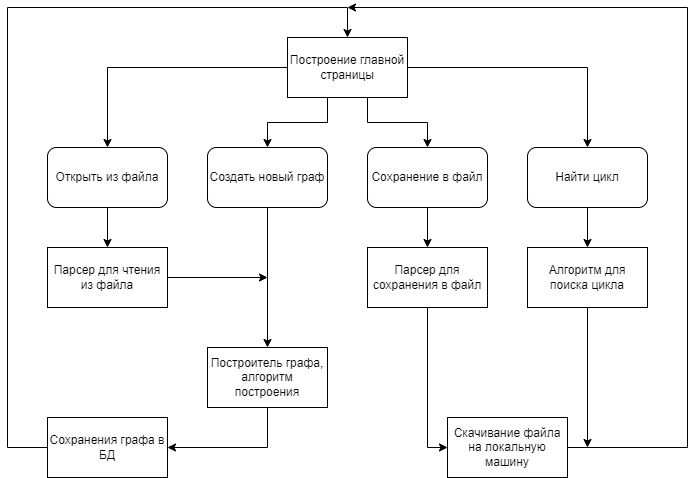
\includegraphics[width=0.7\linewidth]{ResearchNotes/rndhpc_int_edt_2023_01_25/module.png}
    \caption{Концептуальная схема реализации основных сценариев использования разрабатываемого приложения}
    \label{fig:module}
\end{figure}

Среди членов данных класса граф должен быть определён массив узлов графа, а также должны быть реализованы следующие методы:
\begin{description}
\item[make_graph(name)] -- метод, которые преобразует массив в объекте класса в переменную, которую можно сохранить в виде изображения с выбранным расширением;
\item[read_from_aDot(name)] -- метод, читающей из файла с названием name (тип string) данные, затем сохраняет их в поле для узлов;
\item[search_cicles()] -- метод, который находит циклы в графе, возвращает все циклы в виде строки формата \textsf{a-b-c[перенос строки]b-d-e[перенос строки]};
\item[add_eage(e1, e2)] -- метод, добавляющий ребро, исходящее из узла \textsf{e1} и входящее в узел \textsf{e1};
\item[delete_eage(e1, e2)] -- метод, удаляющий ребро, исходящее из узла \textsf{e1} и входящее в узел \textsf{e1};
\item[add_node(node)] -- метод, добавляет узел node;
\item[delete_node(node)] -- метод, удаляющий узел node;
\item[save_into_aDot(name)] -- метод, сохраняет граф в файл с названием name (тип string).
\end{description}

В базе данных необходимо иметь одну таблицу с двумя полями: пользователь и его граф в текстовом виде.\messnote{Очень сомнительно...}

\noteattributes{}
